
The system needs to be calibrated for the current installation height of the Kinect sensor. This is easily done in the Calibration Window which can be started under the System tab in the menu bar. To the left is a thresholded depth image and to the right a histogram. The slider below the histogram adjusts the threshold level. The threshold should be set so that a "normal" person’s chest is not removed by the thresholding. Press Apply to save the changes. 

\begin{figure}[htb]
	\centering
	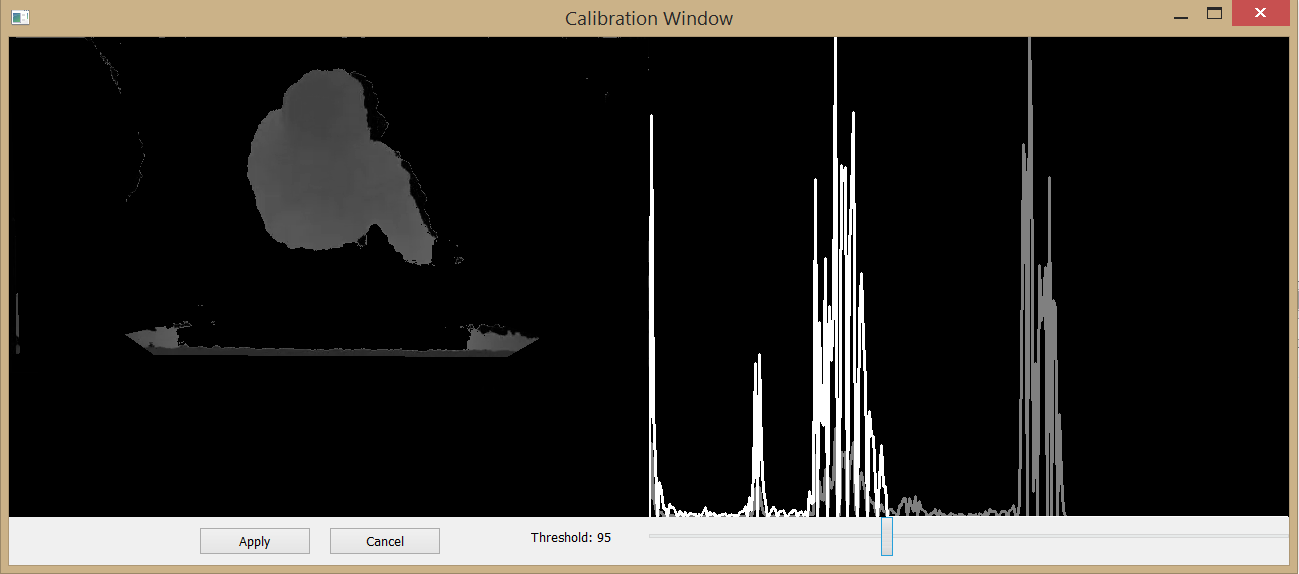
\includegraphics[width=\linewidth]{images/Calibration.png}
	\caption[Overview of the entire system]{\textit{Calibrating the depth threshold of the system. A histogram is shown to help the user. The adjusted histogram is shown in white and the raw histogram in gray.}}
	\label{fig:lowestDistanceOverFloor_calibration}  %Skapar referens till figuren
\end{figure}
